\ifdefined\COMPLETE
\else
    \input{./preambule-sacha-utf8.ltx}
    \begin{document}
\fi

\section{Repères orthonormaux du plan}

Soit $\left(O, \vec{i}, \vec{j} \right)$ un repère orthonormal.

Soit I le point tel que $\overrightarrow{OI} = \vec{i}$\\

Soit J le point tel que $\overrightarrow{OJ} = \vec{j}$\\

% Repère orthonormal
\begin{tikzpicture}[scale=.8]

\tkzInit[xmin=-3,xmax=4, ymin=-2, ymax=4]
\tkzRep[xlabel=$\vec{i}$, ylabel=$\vec{j}$]
\tkzDrawXY [color=black, noticks]%, label={}]
\tkzLabelPoint[color=bistre,below left](0,0){$0$}
\tkzLabelPoint[color=bistre, below](1,0){$I$}
\tkzLabelPoint[color=bistre, left](0,1){$J$}

\end{tikzpicture}

$\left(OI\right) \perp \left(OJ\right) $\\

$OI = OJ = 1 $\\

\subsection{Norme euclidienne d'un vecteur}

Soit $\left(O, \vec{i}, \vec{j} \right)$ un repère orthonormal.

\subsubsection{Définition}

Soit $\vec{u}$ un vecteur.

Soit le point M tel que $\overrightarrow{OM} = \vec{u} $\\

% Norme euclidienne
\begin{tikzpicture}[scale=.8]

\tkzInit[xmin=-3,xmax=10, ymin=-4, ymax=3]
\tkzRep[xlabel=$\vec{i}$, ylabel=$\vec{j}$]
\tkzDrawXY [color=black, noticks]%, label={}]
\tkzLabelPoint[color=bistre,below left](0,0){$0$}
\tkzLabelPoint[color=bistre, below](1,0){$I$}
\tkzLabelPoint[color=bistre, left](0,1){$J$}

\draw [color=blue, thick, ->] (0,0) -- +(6, 2) node [right] {$M$} ; 
\draw [color=blue, thick, ->] (3,-3) -- node[midway,below]{$\vec{u}$} +(6, 2); 

\tkzLabelPoint[color=red, left](0,2){$K$}
\tkzLabelPoint[color=red, below](6,0){$H$}
\end{tikzpicture}

On note $\Vert \vec{u} \Vert $ la norme euclidienne de $\vec{u}$, et on dit que : $\Vert \vec{u} \Vert = OM $\\

\newpage

\subsubsection{Expression de la norme euclidienne d'un vecteur}

Soit $\vec{u}\left(\begin{array}{c} x\\ y \end{array}\right)$\\

Donc $\overrightarrow{OM}\left(\begin{array}{c} x\\ y \end{array}\right)$ et $M\left(x, y\right)$\\

Soit $H$ le projecté orthogonal de M sur $\left(OI\right)$\\

Soit $K$ le projecté orthogonal de M sur $\left(OJ\right)$\\

On peut appliquer le théorème de Pythagore dans le triangle OHM rectangle en H.\\

$ OM^2 = OH^2 + HM^2 $\\

$ OM^2 = OH^2 + OK^2 $\\

$ OM^2 = x^2 + y^2 $\\

$ OM = \sqrt{x^{2} + y^{2}} $\\

Donc, on a pour $\vec{u}\left(\begin{array}{c} x\\ y \end{array}\right)$ : $\Vert \vec{u} \Vert = \sqrt{x^2 + y^2}$\\

\textbf{Exemple}

Pour $\vec{u}\left(\begin{array}{c} 3\\ -4 \end{array}\right)$, on a :

$\Vert \vec{u} \Vert = \sqrt{3^2 + \left(-4\right)^2}$\\

$\Vert \vec{u} \Vert = \sqrt{9 + 16}$\\

$\Vert \vec{u} \Vert = \sqrt{25} $\\

$\Vert \vec{u} \Vert = 5 $\\

\newpage

\subsubsection{Quelques propriétés de la norme euclidienne d'un vecteur}

Soit $\vec{u}$ et $ \vec{v}$ deux vecteurs.

Soit $\lambda \in \R $\\

\begin{itemize}
\item [*] $\Vert \vec{u} \Vert = 0 \Longleftrightarrow \vec{u} = \overrightarrow{0} $\\
\item [*] $\Vert \lambda \vec{u} \Vert = \left|\lambda \right| \Vert \vec{u} \Vert $\\
\item [*] $\Vert \vec{u} + \vec{v} \Vert \leqslant \Vert \vec{u} \Vert + \Vert \vec{v} \Vert $\\
\end{itemize}

\textbf{Remarque}

Il s'agit de l'inégalité triangulaire.

% Propriétés de la norme euclidienne
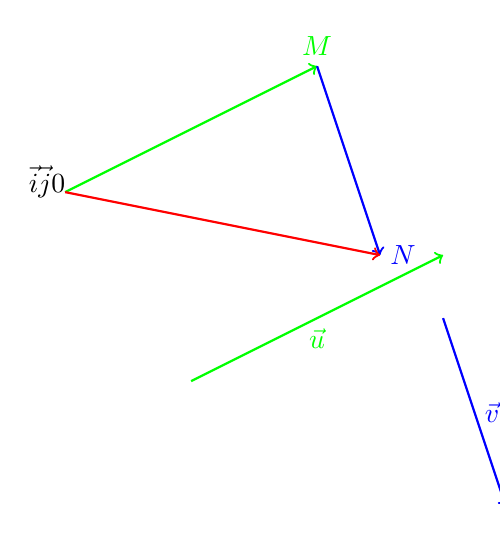
\begin{tikzpicture}[scale=.8]

\tkzInit[xmin=-2,xmax=9, ymin=-6, ymax=3]
\tkzRep[xlabel=$\vec{i}$, ylabel=$\vec{j}$]
\tkzDrawXY [color=black, noticks]%, label={}]
\tkzLabelPoint[color=bistre,below left](0,0){$0$}

\draw [color=green, thick, ->] (2, -3) -- node[midway,below]{$\vec{u}$} +(4, 2) ; 
\draw [color=blue, thick, ->] (6,-2) -- node[midway,right]{$\vec{v}$} +(1, -3) ; 

\draw [color=green, thick, ->] (0,0) -- +(4, 2) node [above] {$M$} ; 
\draw [color=blue, thick, ->] (4,2) -- +(1, -3) node [right] {$N$} ; 
\draw [color=red, thick, ->] (0,0) -- +(5, -1) ;  

\end{tikzpicture}

$ ON \leqslant OM + MN $


\newpage

\subsection{Distance de deux points}

Soit $\left(O, \vec{i}, \vec{j}\right)$ un repère orthonormal.

Soient $A\left(x_A, y_A\right)$ et $B\left(x_B, y_B\right)$\\

$\overrightarrow{AB}\left(\begin{array}{c} x_B - x_A\\ y_B - y_A \end{array}\right)$\\

$AB = \Vert \overrightarrow{AB} \Vert = \sqrt{\left(x_B - x_A\right)^2 + \left(y_B - y_A\right)^2}$\\

\textbf{Exemple}

$A\left(-1,2\right) $ et $B\left(3,-1\right)$\\

% Distance de deux points
\begin{tikzpicture}[scale=.8]

\tkzInit[xmin=-2,xmax=4, ymin=-2, ymax=3]
\tkzRep[xlabel=$\vec{i}$, ylabel=$\vec{j}$]
\tkzDrawXY [very thick, color=black, noticks]%, label={}]
\tkzLabelPoint[color=bistre,below left](0,0){$0$}
\tkzGrid [color=bistre] 

\tkzText(-1, 2){\textcolor{black}{$\times$}} 
\tkzText(3, -1){\textcolor{black}{$\times$}} 

\draw [color=blue, thick] (-1,2) node [above] {$A$} -- (3, -1) node [right] {$B$} ; 


\end{tikzpicture}

$x_B - x_A = 3 + 1 = 4 $\\

$ y_B - y_A = -1 -2 = -3 $\\

$\overrightarrow{AB}\left(\begin{array}{c} 4\\ -3 \end{array}\right)$ \\

$AB = \sqrt{4^2 + \left(-3\right)^2}$\\

$ AB = \sqrt{16 + 9}$\\

$ AB = \sqrt{25} $\\

$ AB = 5 $\\

\textbf{Remarque}

\begin{itemize}
\item[*] Si l'unité est un grand carreau, soit 0,8 cm, alors, la longueur du segment $\left[AB\right] = 5 \time 0,8 = 4 $ cm.
\item[*] Si l'unité est deux petits carreaux, soit 1 cm, alors, la longueur du segment $\left[AB\right] = 5 \time 1 = 5 $ cm.
\end{itemize}

\newpage
\subsection{Exercices}

\subsubsection{Exercice \no 1}

Soit $\left(O, \vec{i}, \vec{j}\right)$ un repère orthonormal.

Soient $A\left(-1,2\right)$ et $B\left(x,-1\right)$\\

Déterminer $x$ pour que $AB = 5$\\

$x_B - x_A = x - \left(-1\right) = x + 1 $\\

$ y_B - y_A = -1 - 2 = -3$. \\

Donc $\overrightarrow{AB}\left(\begin{array}{c} x+1\\ -3 \end{array}\right)$ \\

$ AB = 5 $\\

$ \sqrt{\left(x+1\right)^2 + \left(-3\right)^2} = 5 $\\

$ \sqrt{x^2 + 2x + 10} = 5 $\\

$ x^2 + 2x + 10 = 25 $\\

$ x^2 + 2x - 15 = 0 $\\

$ \left(x+1\right)^2  -16 = 0 $\\

$ \left(x + 1 + 4\right)\left(x+1-4\right) = 0 $\\

$ \left(x+5\right)\left(x-3\right) = 0 $\\

On trouve 2 valeurs à $x$, donc 2 points B : $B_1 \left(-5,1\right)$ et $B_2\left(3,-1\right)$\\

% Ex 1 Arc de cercle
\begin{tikzpicture}[scale=.7]

\tkzInit[xmin=-7,xmax=5, ymin=-4, ymax=3]
\tkzRep[xlabel=$\vec{i}$, ylabel=$\vec{j}$]
\tkzDrawXY [very thick, color=black, noticks]
\tkzLabelPoint[color=bistre,below left](0,0){$0$}

\tkzDefPoint [label=above:$A$](-1,2){A} 
\tkzDefPoint [label=below left:$B_{1}$](-5,-1){B1} 
\tkzDefPoint [label=below right:$B_{2}$](3,-1){B2}

\tkzDrawPoints[size=2,color=black](A,B1,B2)

\tkzCalcLength[cm](A,B1)
\tkzGetLength{rAB}
\draw (B1) arc (217:322:\rAB cm) ; 
\draw [color=black, thick] (B1) -- (A) -- (B2) ;  


\end{tikzpicture}

\newpage
\subsubsection{Exercice \no 2}

Soit $\left(O, \vec{i}, \vec{j}\right)$ un repère orthonormal.

Soient les points $A\left(-2,7\right)$, $B\left(6,1\right)$, $C\left(-3,4\right)$ et $D\left(x,8\right)$\\


1. Soit $\scrC$ le cercle dirconscrit au triangle ABC. Déterminer \textbf{astucieusement} les coordonnées du centre $\Omega$ de $\scrC$. Puis, déterminer le rayon $r$ de $\scrC$\\

% Centre du cercle (astucieusement)
\begin{tikzpicture}[scale=.7]

\tkzInit[xmin=-4,xmax=8, ymin=-2, ymax=9]
\tkzRep[xlabel=$\vec{i}$, ylabel=$\vec{j}$]
\tkzDrawXY [very thick, color=black, noticks]%, label={}]
\tkzLabelPoint[color=bistre,below left](0,0){$0$}
% \tkzGrid [color=bistre] 

\tkzDefPoint [label=left:$A$](-2,7){A} 
\tkzDefPoint [label=right:$B$](6,1){B} 
\tkzDefPoint [label=left:$C$](-3,4){C}
\tkzDefPoint [label=above left:$D_{1}$](-1,8){D1} 
\tkzDefPoint [label=above right:$D_{2}$](5,8){D2}
\tkzDefPoint[label=above right:$\Omega$](2, 4){O} 
\tkzDrawPoints[size=2,color=black](A,B,C,D1,D2,O)

\tkzCalcLength[cm](O,A)
\tkzGetLength{rOB}
\tkzDrawCircle[R](O,\rOB cm)
\draw [color=black, thick] (A) -- (B) -- (C) -- cycle ; 
\draw [color=blue, thick] (A) -- (D1) -- (B) ;
\draw [color=blue] (-1.2,7.8) -- (-1,7.6) -- (-0.8,7.8) ;
\draw [color=red, thick] (A) -- (D2) -- (B) ;  
\draw [color=blue] (-1.2,7.8) -- (-1,7.6) -- (-0.8,7.8) ;
\draw [color=red] (4.75,7.93) -- (4.8,7.7 ) -- (5.05, 7.75) ;  

\tkzDefPoint [label=below:$-3$](-3,0){Xc} 
\tkzDefPoint [label=below:$-2$](-2,0){Xa} 
\tkzDefPoint [label=below:$6$](6,0){Xb} 
\tkzDefPoint [label=left:$4$](0,4){Yc} 
\tkzDefPoint [label=right:$7$](0,7){Ya} 

\tkzDrawPoints[size=2,color=black](Xa,Xb,Xc,Ya,Yc)

\end{tikzpicture}\\



1. Montrons que ABC est un triangle rectangle en C.\\

$\overrightarrow{AB}\left(\begin{array}{c} 8\\ -6 \end{array}\right)$\\

$ AB^2 = 8^2 + \left(-6\right)^2$\\

$ AB^2 = 64 + 36 $\\

$ AB^2 = 100 $\\

$\overrightarrow{CA}\left(\begin{array}{c} 1 \\ 3 \end{array}\right)$ et $\overrightarrow{CB}\left(\begin{array}{c} 9\\ -3 \end{array}\right)$\\

$ CA^2 + CB^2 = 1^2 + 3^2 + 9^2 + \left(-3\right)^2 $\\

$ CA^2 + CB^2 = 1 + 9 + 81 + 9 $\\

$ CA^2 + CB^2 = 100 $\\

On a $ AB^2 = CA^2 + CB^2 $\\

D'après la réciproque du théorème de Pythagore, ABC est un triangle rectangle en C.

Le centre $\Omega$ de $\scrC$ est le milieu de $\left[AB\right]$ car ABC est rectangle en C.\\

$\dfrac{x_A + x_B}{2} = \dfrac{4}{2} = 2$\\

$ \dfrac{y_A + y_B}{2} = \dfrac{8}{2} = 4$\\

On a donc $\Omega \left(2,4\right)$\\

On a $r = \Omega A$\\

$\overrightarrow{\Omega A}\left(\begin{array}{c} -4\\ 3 \end{array}\right)$\\

$\Vert \overrightarrow{\Omega A} \Vert = \sqrt{\left(-4\right)^2 + 3^2} $\\

$\Vert \overrightarrow{\Omega A} \Vert = \sqrt{16 + 9} $\\

$\Vert \overrightarrow{\Omega A} \Vert = \sqrt{25}$\\

$\Vert \overrightarrow{\Omega A} \Vert = 5 $\\

Donc $r=5$


\newpage


2. Déterminer $x$ pour que le triangle ABD soit rectangle en D.

On trouvera deux valeurs de x et donc deux points D : $D_1$ et $D_2$\\

Déterminer $AD_1$ et $BD_1$, puis $AD_2$ et $BD_2$\\

Que remarque-t-on ?\\

On a : $\overrightarrow{DA}\left(\begin{array}{c} -2-x\\ -1 \end{array}\right)$ et $\overrightarrow{DB}\left(\begin{array}{c} 6-x\\ -7 \end{array}\right)$\\

ABD est un triangle rectangle en D.

$ DA^2 + DB^2 = AB^2 $\\

$ \left(-x-2\right)^2 + \left(-1\right)^2 + \left(-x + 6\right)^2 + \left(-7\right)^2 = 100 $\\

$ x^2 + 4x + 4 + 1 + x^2 - 12x + 36 + 49 = 100 $\\

$ 2x^2 - 8x + 90 = 100 $\\

$ 2x^2 - 8x - 10 = 0 $\\

$ 2\left(x^2 - 4x - 5\right) = 0 $\\

$ 2\left[\left(x-2\right)^2 - 9\right] = 0 $\\

$ 2 \left[\left(x - 2 - 3\right)\left(x - 2 + 3\right)\right] = 0 $\\

$ 2\left(x-5\right)\left(x + 1 \right) = 0 $\\

\begin{tabular}{lll}
$x-5 = 0$ & ou & $x+1 = 0$ \\
$ x = 5 $ & ou & $x = -1$ \\
\end{tabular}
\\

$ D_1\left(-1,8\right) $ et $D_2\left(5,8\right)$\\

On a : $\overrightarrow{AD_1}\left(\begin{array}{c} 1\\ 1 \end{array}\right)$, $\overrightarrow{BD_1}\left(\begin{array}{c} -7\\ 7 \end{array}\right)$, $\overrightarrow{AD_2}\left(\begin{array}{c} 7\\ -1 \end{array}\right)$, $\overrightarrow{BD_2}\left(\begin{array}{c} -1\\ 7 \end{array}\right)$\\

On a alors : 
\\
\begin{itemize}
\item [*] $ AD_1 = \sqrt{1^2 + 1^2} = \sqrt{2} $\\
\item [*] $ BD_1 = \sqrt{\left(-7\right)^2 + 7^2} $\\
\item [*] $ AD_2 = \sqrt{7^2 + 1^2} = \sqrt{50} = 5\sqrt{2} $\\
\item [*] $ BD_2 = \sqrt{\left(-1\right)^2 + 7^2} = \sqrt{50} = 5\sqrt{2} $\\
\end{itemize}

Donc $ABD_2$ est un triangle isocèle rectangle.


\ifdefined\COMPLETE
\else
    \end{document}
\fi
